\section{Исследовательская часть}

В данном разделе представлены результаты исследований, проведённых для оценки производительности системы при увеличении объёма данных, анализа скорости получения ответа в зависимости от количества одновременных запросов, а также сравнения скорости обработки с использованием кэширования и без него.

\subsection{Технические характеристики}

Исследования проводилось на устройстве со следующими техническими характеристиками:

\begin{itemize}[label=---]
	\item операционная система macOS 14.6.1~\cite{macos};
	
	\item оперативная память (RAM) 16 ГБ;
	
	\item процессор (CPU) 2 ГГц 4‑ядерный Intel Core i5 (8 логических ядер)~\cite{intel}.
	
\end{itemize}

Во время проведения исследования, устройство было подключено к сети электропитания и не было нагружено сторонними приложениями, за исключением встроенных приложений окружения.

\subsubsection*{\normalsize  Влияние объема данных на время выполнения}


В таблице~\ref{operation-times} приведены результаты исследования времени выполнения операций для различных количеств пользователей в секундах. На рисунке~\ref{grp:dr} изображено графическое представление данных из таблицы~\ref{operation-times}.

\newpage
\begin{table}[ht!]
	\begin{center}
		\caption{Время выполнения операций для различных количеств пользователей}
		\begin{tabular}{ ||p{3.5cm}|r|r|r|r||  }
			\hline
			Количество пользователей & INSERT & UPDATE & DELETE & SELECT \\[1.5ex]
			\hline\hline
			10  & 0.008671  & 0.001736 & 0.001214  & 0.000585  \\
			25  & 0.011783 & 0.004547  & 0.003441  & 0.000304  \\
			50  & 0.018182  & 0.009041  & 0.005436  & 0.000386  \\
			100 & 0.037794 & 0.017999  & 0.011490  & 0.000625  \\
			250 & 0.123677 & 0.052245  & 0.029886  & 0.000983  \\
			500 & 0.185770  & 0.093386  & 0.055787 & 0.001626  \\
			750 & 0.204760 & 0.179636  & 0.091073  & 0.002351 \\
			1000 & 0.252232  & 0.206964 & 0.126073 & 0.003015  \\
			\hline
		\end{tabular}
		\label{operation-times}
	\end{center}
\end{table}

\begin{figure}[ht!]
	\begin{center}
		\begin{tikzpicture}
			\begin{axis}[
				legend pos = north west,
				xlabel=количество пользователей,
				ylabel=секунды,
				grid = major,
				major grid style = {lightgray},
				minor grid style = {lightgray!25},
				width = 1.0\textwidth,
				height = 0.7\textwidth,
				scaled y ticks=base 10:2,
				]
				
				\addplot[
				purple,
				semithick,
				mark = o,
				] file {./diag/time-delete-results.txt};
				\addlegendentry{DELETE}
				
				\addplot[
				red,
				semithick,
				mark = +,
				] file {./diag/time-insert-results.txt};
				\addlegendentry{INSERT}
				
				\addplot[
				blue,
				semithick,
				mark = *,
				] file {./diag/time-update-results.txt};
				\addlegendentry{UPDATE}
				
				\addplot[
				darkgray,
				semithick,
				mark = x,
				] file {./diag/time-select-results.txt};
				\addlegendentry{SELECT}
			\end{axis}
		\end{tikzpicture}
	\end{center}
	\caption{Зависимость времени выполнения операций от количества пользователей}
	\label{grp:dr}
\end{figure}

\subsubsection*{\normalsize Влияние количества одновременных запросов на отклик}

В рамках исследования была оценена производительность выборки данных из таблицы User при различных уровнях параллельной нагрузки на базу данных. 
Каждый тест длился 10 секунд, в течение которых пользователи базы данных (клиенты) выполняли запросы.

В таблице~\ref{operation-times2} приведены результаты исследования времени отклика от количества клиентов в миллисекундах. На рисунке~\ref{grp:dr2} изображено графическое представление данных из таблицы~\ref{operation-times2}.


\begin{table}[h!]
	\centering
	\caption{Результаты нагрузочного тестирования}
	\begin{tabular}{|p{3.5cm}|p{4.5cm}|p{3.5cm}|}
		\hline
		\textbf{Количество клиентов} & \textbf{Среднее время отклика (мс)} & \textbf{Количество запросов} \\
		\hline
		1  & 0.272817  & 36\,550 \\
		10 & 1.516456  & 65\,898 \\
		25 & 5.964658  & 41\,914 \\
		50 & 11.333167 & 44\,124 \\
		75 & 13.321161 & 56\,332 \\
		\hline
	\end{tabular}
	\label{operation-times2}
\end{table}

\begin{figure}[ht!]
	\begin{center}
		\begin{tikzpicture}
			\begin{axis}[
				legend pos = north west,
				xlabel=количество клиентов,
				xmin=-1,
				xmax=77,
				ylabel=миллисекунды,
				grid = major,
				major grid style = {lightgray},
				minor grid style = {lightgray!25},
				width = 1.0\textwidth,
				height = 0.5\textwidth,
				scaled y ticks=base 10:0,
				]
				
				\addplot[
				purple,
				semithick,
				mark = o,
				] file {./diag/time-avg-results.txt};
			\end{axis}
		\end{tikzpicture}
	\end{center}
	\caption{Зависимость времени отклика от количества клиентов}
	\label{grp:dr2}
\end{figure}

\subsubsection*{\normalsize Влияние кэширования на скорость запросов}

В рамках исследования была оценена производительность запросов к данным, получаемым из базы данных PostgreSQL и Redis-кэша. 

Основной задачей было извлечение информации о пользователях, родившихся после 1 января 2003 года и имеющих женский пол, с последующей сортировкой по дате рождения.

Для каждого из источников данных были замерены времена отклика на запросы. Каждый запрос к кэшу и базе данных выполнялся 30 раз. Исследование проводилось на протяжении нескольких минут, с интервалом в 5 секунд между запросами. Кэш в Redis хранился в течение 10 секунд.

Среднее время выполнения запросов к Redis-кэшу (Кэш) составило 0.00188 секунды, для базы данных PostgreSQL (БД) -- 0.00246 секунды. На рисунке~\ref{fig:dr3} изображено графическое представление полученных данных. 

\begin{figure}[ht!]
	\begin{center}
		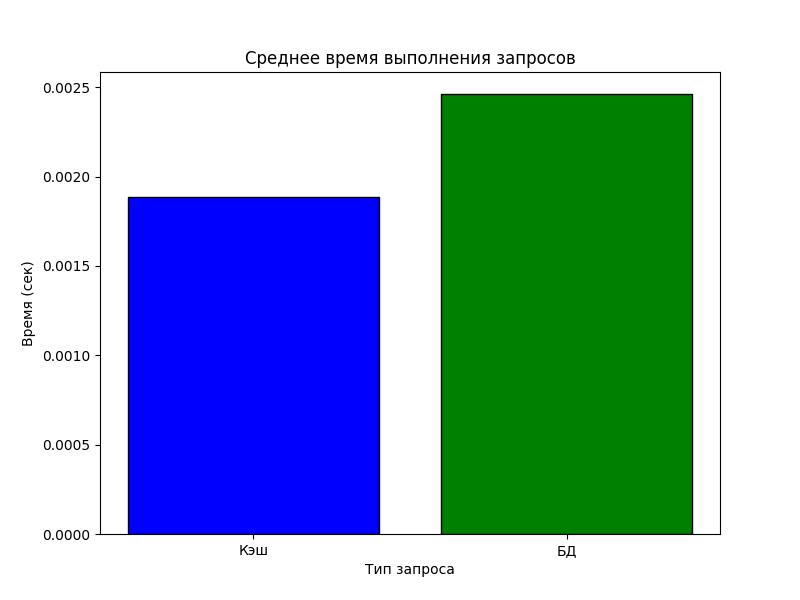
\includegraphics[scale=0.7]{./img/just.png}
	\end{center}
	\caption{Сравнение времени выполнения запросов к кэшу и базе данных}
	\label{fig:dr3}
\end{figure}


\subsection*{Вывод}

Результаты первого исследования показали, что с увеличением числа записей в таблице пользователей время выполнения операций увеличивается:
\begin{itemize}
	\item время выполнения операции INSERT увеличивается с 0.0087 секунд при 10 пользователях до 0.2522 секунд при 1000 пользователях;
	\item время выполнения операции UPDATE увеличивается с 0.0017 секунд при 10 пользователях до 0.2070 секунд при 1000 пользователях;
	\item время выполнения операции DELETE увеличивается с 0.0012 секунд при 10 пользователях до 0.1261 секунд при 1000 пользователях;
	\item время выполнения операции SELECT увеличивается с 0.0006 секунд при 10 пользователях до 0.0030 секунд при 1000 пользователях.
\end{itemize}

Время выполнения операций значительно увеличивается при росте количества записей в таблице, особенно для операций изменения данных (INSERT, UPDATE, DELETE), в то время как операция SELECT остается сравнительно стабильной.

Результаты второго исследования показали, что с увеличением количества клиентов время отклика на запросы также увеличивается. Так, при 10 клиентах среднее время отклика составило 1.5165 миллисекунды, а при 75 клиентах -- 13.3212 миллисекунды. Это свидетельствует о том, что с ростом числа одновременных запросов наблюдается значительное увеличение времени отклика, что указывает на увеличение нагрузки на базу данных.

Результаты третьего исследования показали, что кэширование ускоряет выполнение запросов. Среднее время выполнения запроса к Redis-кэшу составило 0.00188 секунды, что на 0.00058 секунды быстрее, чем запросы к базе данных PostgreSQL, где среднее время составило 0.00246 секунды. Это подтверждает эффективность использования кэширования для ускорения обработки данных.